% Options for packages loaded elsewhere
\PassOptionsToPackage{unicode}{hyperref}
\PassOptionsToPackage{hyphens}{url}
\documentclass[
]{article}
\usepackage{xcolor}
\usepackage{amsmath,amssymb}
\setcounter{secnumdepth}{5}
\usepackage{iftex}
\ifPDFTeX
  \usepackage[T1]{fontenc}
  \usepackage[utf8]{inputenc}
  \usepackage{textcomp} % provide euro and other symbols
\else % if luatex or xetex
  \usepackage{unicode-math} % this also loads fontspec
  \defaultfontfeatures{Scale=MatchLowercase}
  \defaultfontfeatures[\rmfamily]{Ligatures=TeX,Scale=1}
\fi
\usepackage{lmodern}
\ifPDFTeX\else
  % xetex/luatex font selection
\fi
% Use upquote if available, for straight quotes in verbatim environments
\IfFileExists{upquote.sty}{\usepackage{upquote}}{}
\IfFileExists{microtype.sty}{% use microtype if available
  \usepackage[]{microtype}
  \UseMicrotypeSet[protrusion]{basicmath} % disable protrusion for tt fonts
}{}
\makeatletter
\@ifundefined{KOMAClassName}{% if non-KOMA class
  \IfFileExists{parskip.sty}{%
    \usepackage{parskip}
  }{% else
    \setlength{\parindent}{0pt}
    \setlength{\parskip}{6pt plus 2pt minus 1pt}}
}{% if KOMA class
  \KOMAoptions{parskip=half}}
\makeatother
\usepackage{color}
\usepackage{fancyvrb}
\newcommand{\VerbBar}{|}
\newcommand{\VERB}{\Verb[commandchars=\\\{\}]}
\DefineVerbatimEnvironment{Highlighting}{Verbatim}{commandchars=\\\{\}}
% Add ',fontsize=\small' for more characters per line
\newenvironment{Shaded}{}{}
\newcommand{\AlertTok}[1]{\textcolor[rgb]{1.00,0.00,0.00}{\textbf{#1}}}
\newcommand{\AnnotationTok}[1]{\textcolor[rgb]{0.38,0.63,0.69}{\textbf{\textit{#1}}}}
\newcommand{\AttributeTok}[1]{\textcolor[rgb]{0.49,0.56,0.16}{#1}}
\newcommand{\BaseNTok}[1]{\textcolor[rgb]{0.25,0.63,0.44}{#1}}
\newcommand{\BuiltInTok}[1]{\textcolor[rgb]{0.00,0.50,0.00}{#1}}
\newcommand{\CharTok}[1]{\textcolor[rgb]{0.25,0.44,0.63}{#1}}
\newcommand{\CommentTok}[1]{\textcolor[rgb]{0.38,0.63,0.69}{\textit{#1}}}
\newcommand{\CommentVarTok}[1]{\textcolor[rgb]{0.38,0.63,0.69}{\textbf{\textit{#1}}}}
\newcommand{\ConstantTok}[1]{\textcolor[rgb]{0.53,0.00,0.00}{#1}}
\newcommand{\ControlFlowTok}[1]{\textcolor[rgb]{0.00,0.44,0.13}{\textbf{#1}}}
\newcommand{\DataTypeTok}[1]{\textcolor[rgb]{0.56,0.13,0.00}{#1}}
\newcommand{\DecValTok}[1]{\textcolor[rgb]{0.25,0.63,0.44}{#1}}
\newcommand{\DocumentationTok}[1]{\textcolor[rgb]{0.73,0.13,0.13}{\textit{#1}}}
\newcommand{\ErrorTok}[1]{\textcolor[rgb]{1.00,0.00,0.00}{\textbf{#1}}}
\newcommand{\ExtensionTok}[1]{#1}
\newcommand{\FloatTok}[1]{\textcolor[rgb]{0.25,0.63,0.44}{#1}}
\newcommand{\FunctionTok}[1]{\textcolor[rgb]{0.02,0.16,0.49}{#1}}
\newcommand{\ImportTok}[1]{\textcolor[rgb]{0.00,0.50,0.00}{\textbf{#1}}}
\newcommand{\InformationTok}[1]{\textcolor[rgb]{0.38,0.63,0.69}{\textbf{\textit{#1}}}}
\newcommand{\KeywordTok}[1]{\textcolor[rgb]{0.00,0.44,0.13}{\textbf{#1}}}
\newcommand{\NormalTok}[1]{#1}
\newcommand{\OperatorTok}[1]{\textcolor[rgb]{0.40,0.40,0.40}{#1}}
\newcommand{\OtherTok}[1]{\textcolor[rgb]{0.00,0.44,0.13}{#1}}
\newcommand{\PreprocessorTok}[1]{\textcolor[rgb]{0.74,0.48,0.00}{#1}}
\newcommand{\RegionMarkerTok}[1]{#1}
\newcommand{\SpecialCharTok}[1]{\textcolor[rgb]{0.25,0.44,0.63}{#1}}
\newcommand{\SpecialStringTok}[1]{\textcolor[rgb]{0.73,0.40,0.53}{#1}}
\newcommand{\StringTok}[1]{\textcolor[rgb]{0.25,0.44,0.63}{#1}}
\newcommand{\VariableTok}[1]{\textcolor[rgb]{0.10,0.09,0.49}{#1}}
\newcommand{\VerbatimStringTok}[1]{\textcolor[rgb]{0.25,0.44,0.63}{#1}}
\newcommand{\WarningTok}[1]{\textcolor[rgb]{0.38,0.63,0.69}{\textbf{\textit{#1}}}}
\usepackage{longtable,booktabs,array}
\newcounter{none} % for unnumbered tables
\usepackage{calc} % for calculating minipage widths
% Correct order of tables after \paragraph or \subparagraph
\usepackage{etoolbox}
\makeatletter
\patchcmd\longtable{\par}{\if@noskipsec\mbox{}\fi\par}{}{}
\makeatother
% Allow footnotes in longtable head/foot
\IfFileExists{footnotehyper.sty}{\usepackage{footnotehyper}}{\usepackage{footnote}}
\makesavenoteenv{longtable}
\usepackage{graphicx}
\makeatletter
\newsavebox\pandoc@box
\newcommand*\pandocbounded[1]{% scales image to fit in text height/width
  \sbox\pandoc@box{#1}%
  \Gscale@div\@tempa{\textheight}{\dimexpr\ht\pandoc@box+\dp\pandoc@box\relax}%
  \Gscale@div\@tempb{\linewidth}{\wd\pandoc@box}%
  \ifdim\@tempb\p@<\@tempa\p@\let\@tempa\@tempb\fi% select the smaller of both
  \ifdim\@tempa\p@<\p@\scalebox{\@tempa}{\usebox\pandoc@box}%
  \else\usebox{\pandoc@box}%
  \fi%
}
% Set default figure placement to htbp
\def\fps@figure{htbp}
\makeatother
\setlength{\emergencystretch}{3em} % prevent overfull lines
\providecommand{\tightlist}{%
  \setlength{\itemsep}{0pt}\setlength{\parskip}{0pt}}
\usepackage{bookmark}
\IfFileExists{xurl.sty}{\usepackage{xurl}}{} % add URL line breaks if available
\urlstyle{same}
\hypersetup{
  pdftitle={Prahari --- Complete Technical Documentation},
  pdfauthor={FinSpark'26 · Bank of Maharashtra · Problem Statement 1 --- Privileged Access Misuse \& Insider Threat Detection},
  hidelinks,
  pdfcreator={LaTeX via pandoc}}

\title{Prahari --- Complete Technical Documentation}
\usepackage{etoolbox}
\makeatletter
\providecommand{\subtitle}[1]{% add subtitle to \maketitle
  \apptocmd{\@title}{\par {\large #1 \par}}{}{}
}
\makeatother
\subtitle{Privileged-Access Insider-Threat Detection \& Management for
Banks}
\author{FinSpark'26 · Bank of Maharashtra · Problem Statement 1 ---
Privileged Access Misuse \& Insider Threat Detection}
\date{Repository: github.com/positromen/FinSpark-26-Trial}

\begin{document}
\maketitle

{
\setcounter{tocdepth}{3}
\tableofcontents
}
\section{Executive Summary}\label{executive-summary}

\textbf{Prahari} (``sentinel'') is a Privileged Access Management (PAM)
\emph{and} insider-threat detection platform for banks. It sits between
privileged staff --- DBAs, sysadmins, network and application admins,
and vendors --- and critical systems, and does four things for every
privileged session:

\begin{itemize}
\tightlist
\item
  \textbf{Watches} every privileged action as a normalized,
  \textbf{recorded} session with a replayable command trail.
\item
  \textbf{Scores} each session \textbf{0--100 in real time}, fusing a
  rule engine with AI behavioural analytics (UEBA) and peer comparison,
  always with a human-readable \emph{why}.
\item
  \textbf{Responds} adaptively --- \textbf{ALLOW / STEP-UP MFA /
  MAKER-CHECKER / BLOCK} --- tagged with the detected \textbf{insider
  type}.
\item
  \textbf{Protects} its own credentials and audit log with \textbf{NIST
  post-quantum cryptography} (ML-KEM-768 vault and ML-DSA-65 signed
  hash-chain).
\end{itemize}

It ships as a real two-sided product: an \textbf{Employee Portal} where
staff act and enforcement happens live, and a \textbf{SOC Console} where
analysts watch, replay sessions, review access, and verify the audit
chain. It runs \textbf{fully offline} on SQLite and is one connection
string away from PostgreSQL.

\textbf{All six judged outcomes are delivered:} detect misuse of
privileged accounts; identify insider threats in real time; AI-driven
behavioural analysis; risk-based access control; protect critical
administrative systems; and quantum-proof cryptography for credentials
and audit artefacts.

\section{Problem and Context}\label{problem-and-context}

Traditional bank security --- firewalls, antivirus, perimeter IAM --- is
built for \textbf{outsiders}. It is largely blind to a \textbf{trusted
insider} who already holds privileged access. Problem Statement 1 names
three insider archetypes explicitly, all of which must be demonstrable:
\textbf{malicious}, \textbf{negligent}, and \textbf{compromised}.

Common failure modes in privileged access:

\begin{itemize}
\tightlist
\item
  \textbf{Dormant and vendor accounts} never deactivated --- a classic
  entry point.
\item
  \textbf{Privilege escalation} performed outside the grant process.
\item
  \textbf{Mass export} of customer records; \textbf{after-hours} bulk
  access.
\item
  \textbf{Expired vendor access} still in daily use (negligence).
\item
  \textbf{Account takeover} --- new geography or device, inhuman action
  pace (compromise).
\item
  \textbf{Tamperable audit logs} --- the insider edits the evidence.
\item
  \textbf{``Harvest-now, decrypt-later''} --- credentials and evidence
  encrypted with classical cryptography today may be broken by future
  quantum computers.
\end{itemize}

\textbf{Why we chose it.} It carries the highest business impact for a
bank --- fraud loss, RBI compliance, and customer trust --- and it lets
us combine real-time AI/UEBA, PAM controls, and post-quantum
cryptography into one coherent, defensible solution.

\section{Solution Overview}\label{solution-overview}

Prahari performs four steps, in order, for every privileged session:
record and normalize the activity, score it, enforce an adaptive
response, and protect the resulting evidence with post-quantum
cryptography. Two role-based experiences sit behind one login:

\begin{itemize}
\tightlist
\item
  \textbf{Employee Portal} --- a privileged-access console where staff
  perform actions (query, file access, configuration change, privilege
  escalation, bulk export). Each action is scored and \textbf{enforced
  live} before it takes effect.
\item
  \textbf{SOC Console} --- the analyst's control room: live sessions, a
  risk gauge, insider-type-tagged alerts, a why-flagged panel, a session
  timeline, \textbf{privileged-session replay}, a risk heatmap, a
  \textbf{PAM access review}, and post-quantum audit \textbf{verify /
  tamper} controls.
\end{itemize}

\section{System Architecture}\label{system-architecture}

Six modules carry activity from ingestion through analytics, scoring,
response, and the post-quantum security layer.

\begin{figure}
\centering
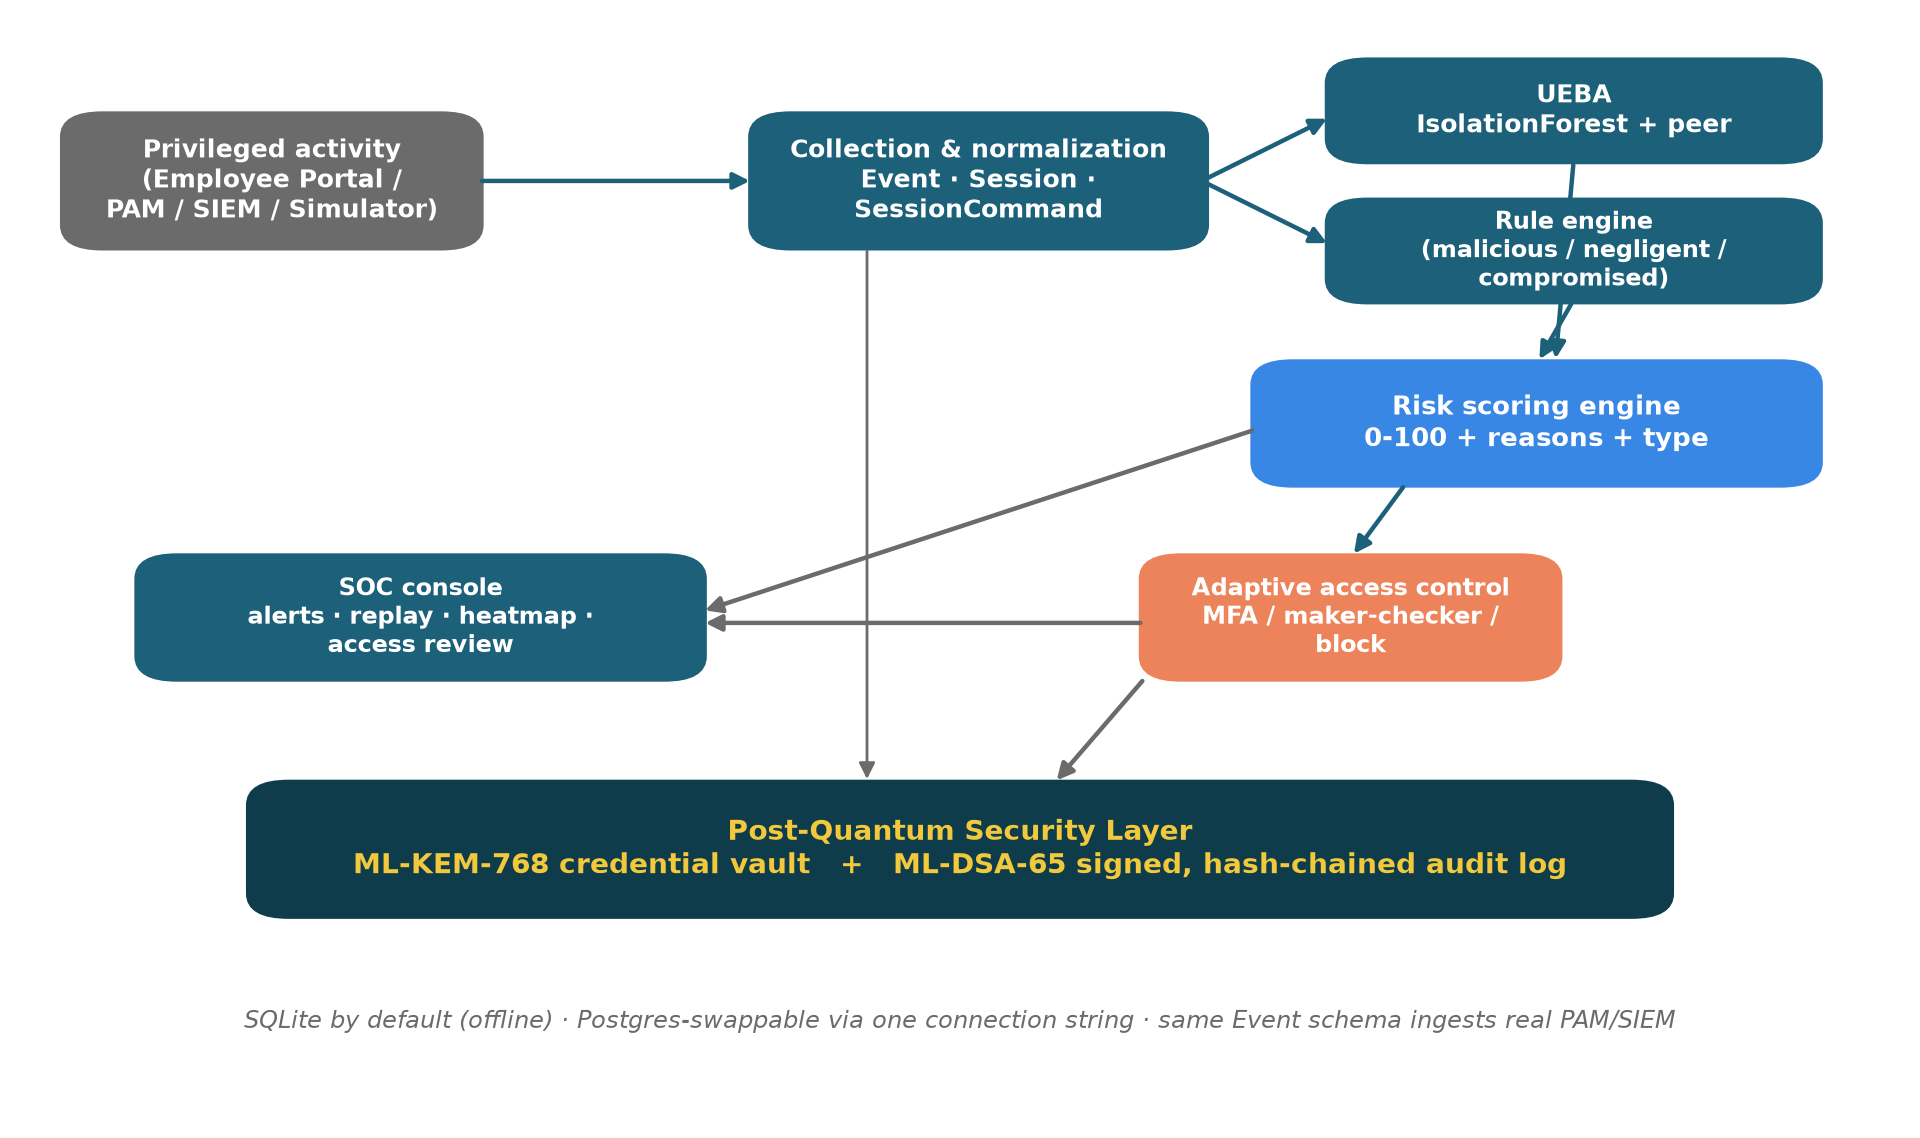
\includegraphics[width=1\linewidth,height=\textheight,keepaspectratio,alt={Prahari system architecture --- six modules from ingestion to the post-quantum security layer.}]{img/architecture.png}
\caption{Prahari system architecture --- six modules from ingestion to
the post-quantum security layer.}
\end{figure}

The Employee Portal, and in production any PAM/SIEM feed, map onto the
same normalized \texttt{Event} schema; the built-in simulator produces
the same shape for the demo.

\textbf{Technology stack}

{\def\LTcaptype{none} % do not increment counter
\begin{longtable}[]{@{}
  >{\raggedright\arraybackslash}p{(\linewidth - 2\tabcolsep) * \real{0.5000}}
  >{\raggedright\arraybackslash}p{(\linewidth - 2\tabcolsep) * \real{0.5000}}@{}}
\toprule\noalign{}
\begin{minipage}[b]{\linewidth}\raggedright
Layer
\end{minipage} & \begin{minipage}[b]{\linewidth}\raggedright
Choice
\end{minipage} \\
\midrule\noalign{}
\endhead
\bottomrule\noalign{}
\endlastfoot
Backend / API & Python 3.14, FastAPI + Uvicorn \\
Storage & SQLAlchemy ORM · SQLite (default) -\textgreater{}
PostgreSQL-swappable \\
AI / UEBA & scikit-learn IsolationForest + peer baselining \\
Post-quantum crypto & liboqs-python --- ML-KEM-768 (FIPS 203), ML-DSA-65
(FIPS 204); AES-256-GCM \\
Authentication & PBKDF2-HMAC-SHA256 passwords + HMAC-signed tokens
(standard library) \\
Real-time & FastAPI WebSocket \\
Frontend & React 19 + Vite + Tailwind 4 (+ Recharts) \\
Packaging & Docker + docker-compose · run.ps1 / run.sh \\
Testing & pytest (31 tests) \\
\end{longtable}
}

\section{Data Model}\label{data-model}

Seven ORM entities capture the workforce, their recorded sessions and
actions, the detection output, and the post-quantum artefacts.

\begin{figure}
\centering
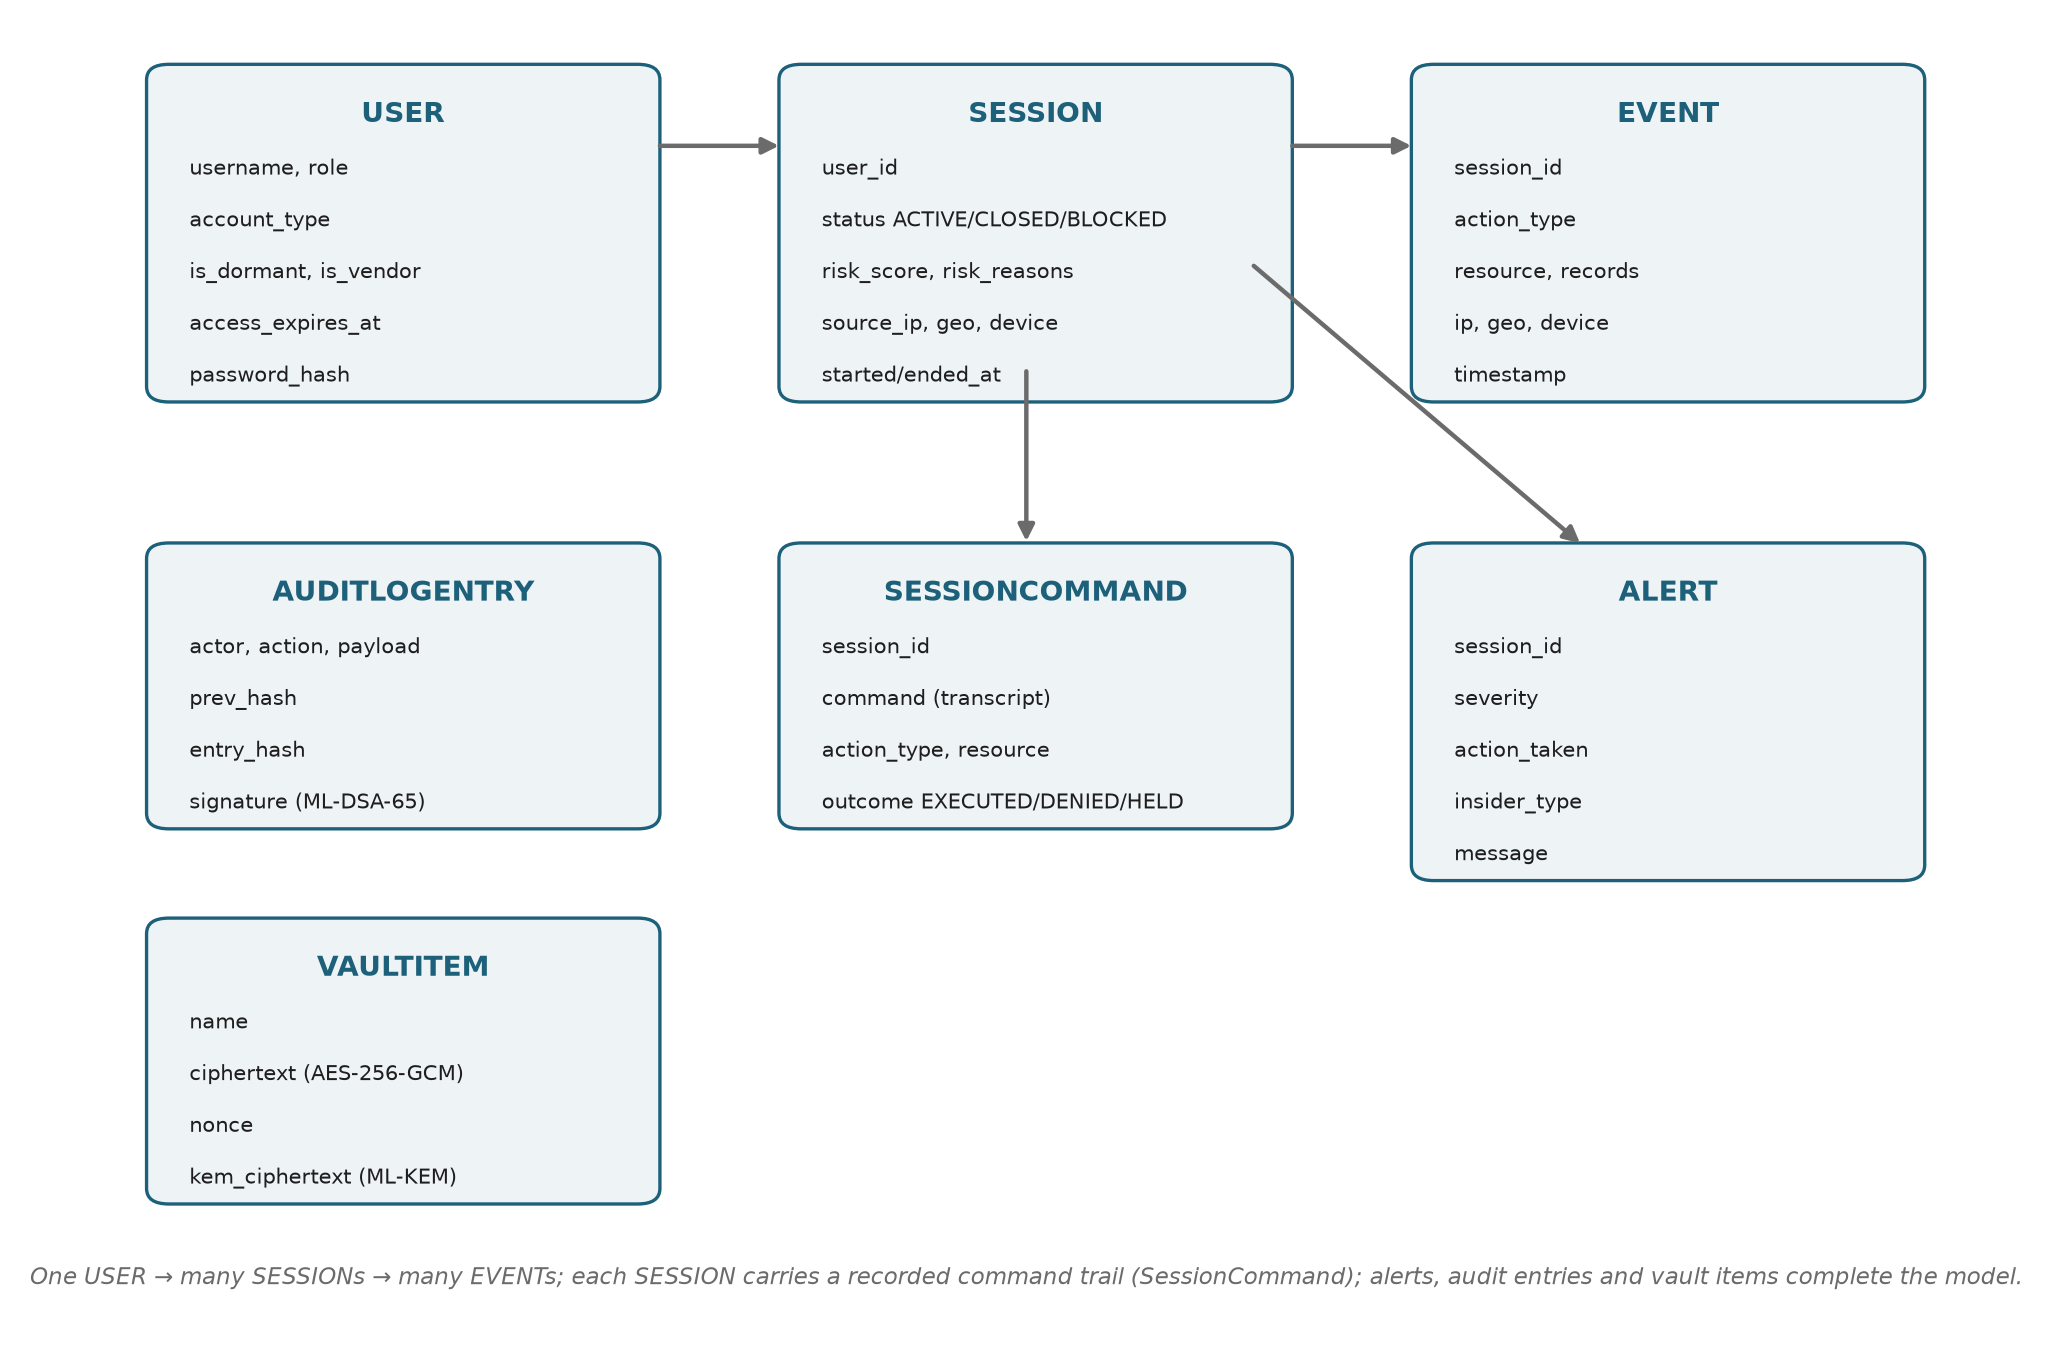
\includegraphics[width=1\linewidth,height=\textheight,keepaspectratio,alt={Entity model --- users, sessions, events, recorded commands, alerts, audit entries and vault items.}]{img/datamodel.png}
\caption{Entity model --- users, sessions, events, recorded commands,
alerts, audit entries and vault items.}
\end{figure}

\texttt{SessionCommand} is the \textbf{privileged-session recording}:
every action writes a realistic command line (for example,
\texttt{psql\ core-banking-db\ -c\ "COPY\ customers\ TO\ \textquotesingle{}/tmp/out.csv\textquotesingle{}\ CSV;"\ -\/-\ 5000\ rows})
with an outcome, so a session replays like a terminal transcript.

\textbf{Seeded cast} (all password \texttt{prahari123}):

{\def\LTcaptype{none} % do not increment counter
\begin{longtable}[]{@{}
  >{\raggedright\arraybackslash}p{(\linewidth - 4\tabcolsep) * \real{0.3333}}
  >{\raggedright\arraybackslash}p{(\linewidth - 4\tabcolsep) * \real{0.3333}}
  >{\raggedright\arraybackslash}p{(\linewidth - 4\tabcolsep) * \real{0.3333}}@{}}
\toprule\noalign{}
\begin{minipage}[b]{\linewidth}\raggedright
Username
\end{minipage} & \begin{minipage}[b]{\linewidth}\raggedright
Role
\end{minipage} & \begin{minipage}[b]{\linewidth}\raggedright
Notes
\end{minipage} \\
\midrule\noalign{}
\endhead
\bottomrule\noalign{}
\endlastfoot
rmehta, spatil & DBA & permanent staff \\
akulkarni, pjoshi & SYSADMIN & permanent staff (akulkarni =
compromised-scenario subject) \\
vdeshmukh & NET\_ADMIN & permanent staff \\
nshinde & APP\_ADMIN & permanent staff \\
ext\_dsouza & CONTRACTOR & dormant vendor, access expired 120 days
-\textgreater{} malicious attacker \\
ext\_rao & CONTRACTOR & active vendor, access expired 18 days
-\textgreater{} negligent subject \\
soc\_admin & SOC\_ANALYST & logs into the SOC console (account\_type =
ANALYST) \\
\end{longtable}
}

\section{Detection Engine}\label{detection-engine}

Two detectors feed one scorer.

\subsection{Rule engine}\label{rule-engine}

Each rule returns a \textbf{reason}, a \textbf{weight}, and an
\textbf{insider\_type} tag.

{\def\LTcaptype{none} % do not increment counter
\begin{longtable}[]{@{}
  >{\raggedright\arraybackslash}p{(\linewidth - 6\tabcolsep) * \real{0.2500}}
  >{\raggedright\arraybackslash}p{(\linewidth - 6\tabcolsep) * \real{0.2500}}
  >{\raggedright\arraybackslash}p{(\linewidth - 6\tabcolsep) * \real{0.2500}}
  >{\raggedright\arraybackslash}p{(\linewidth - 6\tabcolsep) * \real{0.2500}}@{}}
\toprule\noalign{}
\begin{minipage}[b]{\linewidth}\raggedright
Rule
\end{minipage} & \begin{minipage}[b]{\linewidth}\raggedright
Fires when
\end{minipage} & \begin{minipage}[b]{\linewidth}\raggedright
Weight
\end{minipage} & \begin{minipage}[b]{\linewidth}\raggedright
Type
\end{minipage} \\
\midrule\noalign{}
\endhead
\bottomrule\noalign{}
\endlastfoot
DORMANT\_REACTIVATION & a dormant account logs in & 30 & malicious \\
PRIVILEGE\_ESCALATION & a privilege-change event occurs & 25 &
malicious \\
AFTER\_HOURS\_ACCESS & activity between 00:00 and 06:00 & 20 &
malicious \\
MASS\_EXPORT & at least 1000 records in one session & 30 & malicious \\
NO\_BUSINESS\_RELATIONSHIP & resource outside the user's role & 15 &
malicious \\
NEW\_GEO & login location is not the home location & 16 & compromised \\
NEW\_DEVICE & unrecognized device \textbf{with} a foreign location & 12
& compromised \\
ATYPICAL\_HOUR & login in an off-shift hour (06, 20--23) & 8 &
compromised \\
RAPID\_FIRE & at least 5 actions within 180 seconds (inhuman pace) & 8 &
compromised \\
EXPIRED\_ACCESS\_IN\_USE & the user's access grant has lapsed & 30 &
negligent \\
UNMANAGED\_DEVICE & sensitive data from a new device at the
\textbf{home} location & 30 & negligent \\
\end{longtable}
}

The \textbf{dominant insider type} of a session is the category carrying
the most rule weight (tie-break priority: malicious, then compromised,
then negligent).

\textbf{Device disambiguation.} A new device \emph{with} a foreign
geography reads as account takeover (\texttt{NEW\_DEVICE}, compromised);
a new device from the \emph{home} location reads as a personal,
unmanaged laptop (\texttt{UNMANAGED\_DEVICE}, negligent). This keeps the
two families cleanly separated.

\subsection{UEBA --- behavioural
analytics}\label{ueba-behavioural-analytics}

Every session becomes a 7-feature vector:
\texttt{login\_hour,\ event\_count,\ total\_records,\ distinct\_resources,\ config\_changes,\ offsite\_ip,\ new\_device}.

\begin{itemize}
\tightlist
\item
  An \textbf{IsolationForest} (100 trees) is trained on \textbf{closed
  historical sessions}, including \textbf{cumulative prefixes} of each
  session --- so live sessions (which arrive one action at a time) are
  in-distribution and normal early activity is not flagged merely for
  being short.
\item
  The raw anomaly is normalized to \textbf{0--100} against the baseline
  distribution (median maps to 0, first percentile maps to 100).
\item
  \textbf{Peer comparison} measures the session's record volume against
  the same-role average --- for example, ``5000× more records than
  CONTRACTOR peers''.
\end{itemize}

\subsection{Risk scoring}\label{risk-scoring}

The final score fuses the two detectors:

\[\text{score} = \min\!\big(\; \text{rule\_weight (capped at 80)} \;+\; 0.25 \times \text{UEBA\_anomaly} \;+\; \text{peer\_bonus (10 if} \geq 5\times \text{peers)}, \; 100 \big)\]

UEBA is a \textbf{secondary nudge} (at most 25 points): the stable,
explainable rule engine sets the band; the behavioural model refines
within it. Every score ships a reason list (the ``why-flagged'' panel)
and the insider type.

\begin{figure}
\centering
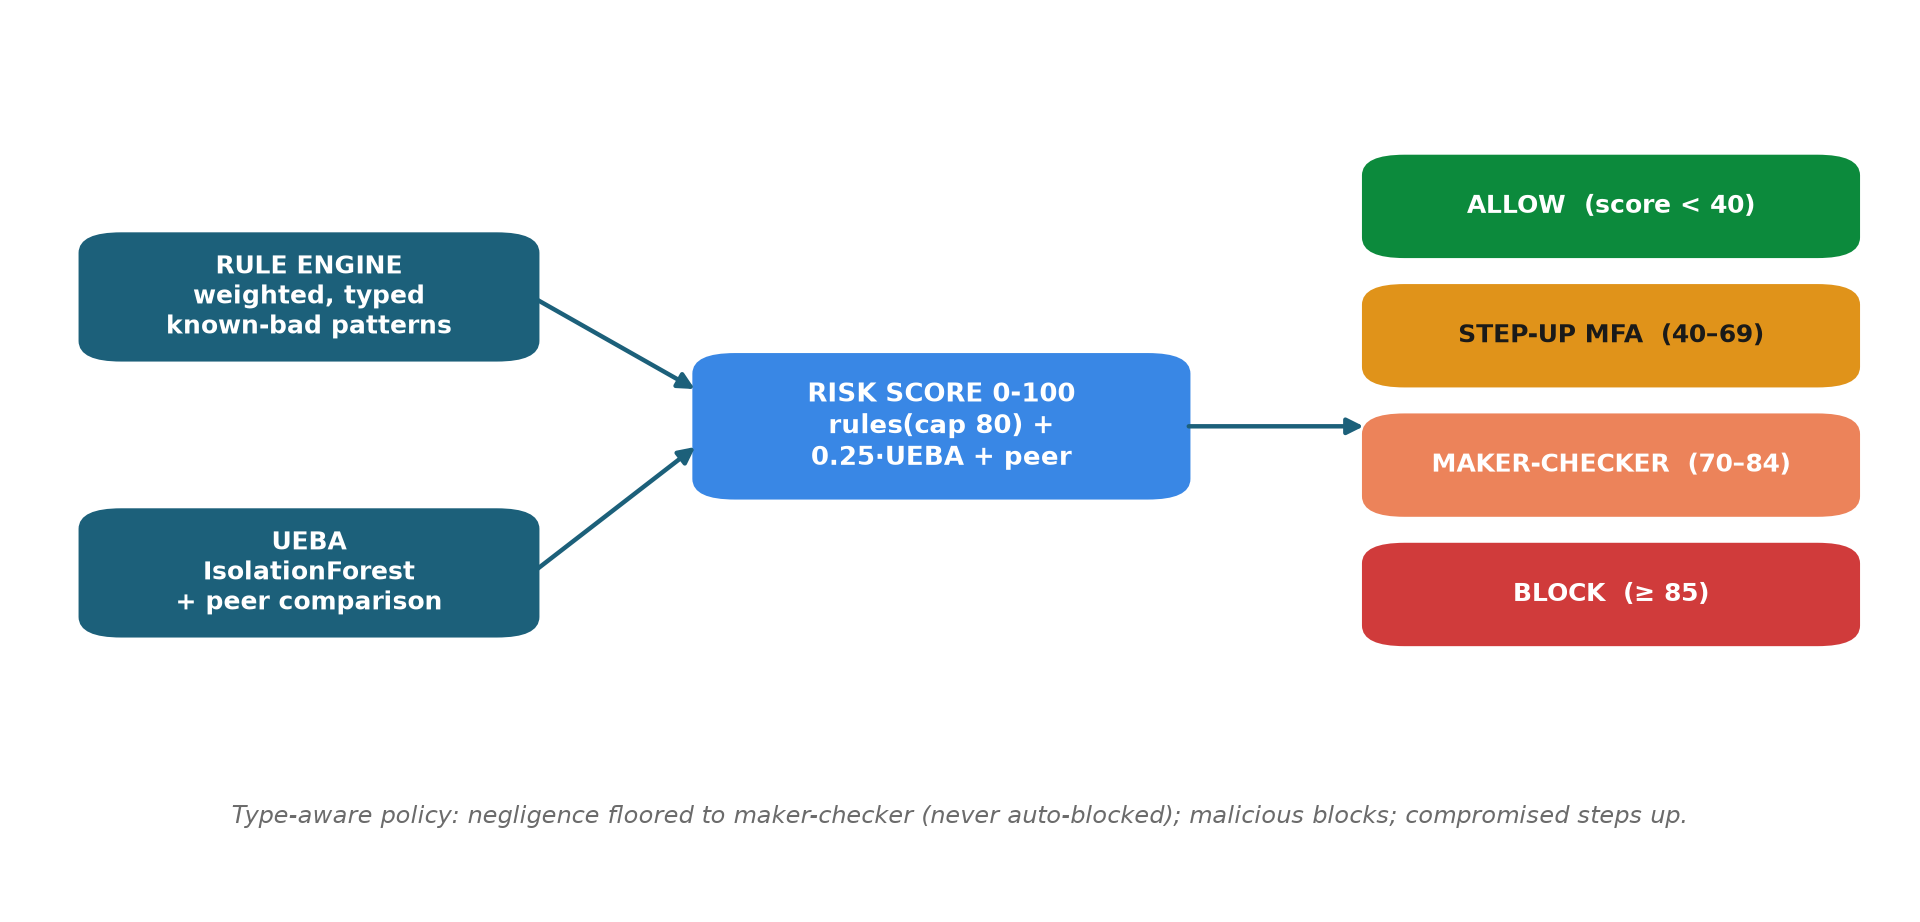
\includegraphics[width=1\linewidth,height=\textheight,keepaspectratio,alt={Scoring pipeline --- rules and UEBA fuse into a 0--100 score that maps onto the response ladder.}]{img/scoring.png}
\caption{Scoring pipeline --- rules and UEBA fuse into a 0--100 score
that maps onto the response ladder.}
\end{figure}

\section{The Three Insider Types}\label{the-three-insider-types}

Three scripted scenarios (one SOC button each) prove three
\textbf{distinct} response paths. The behaviour is verified live and by
automated tests on an independent random seed.

\begin{figure}
\centering
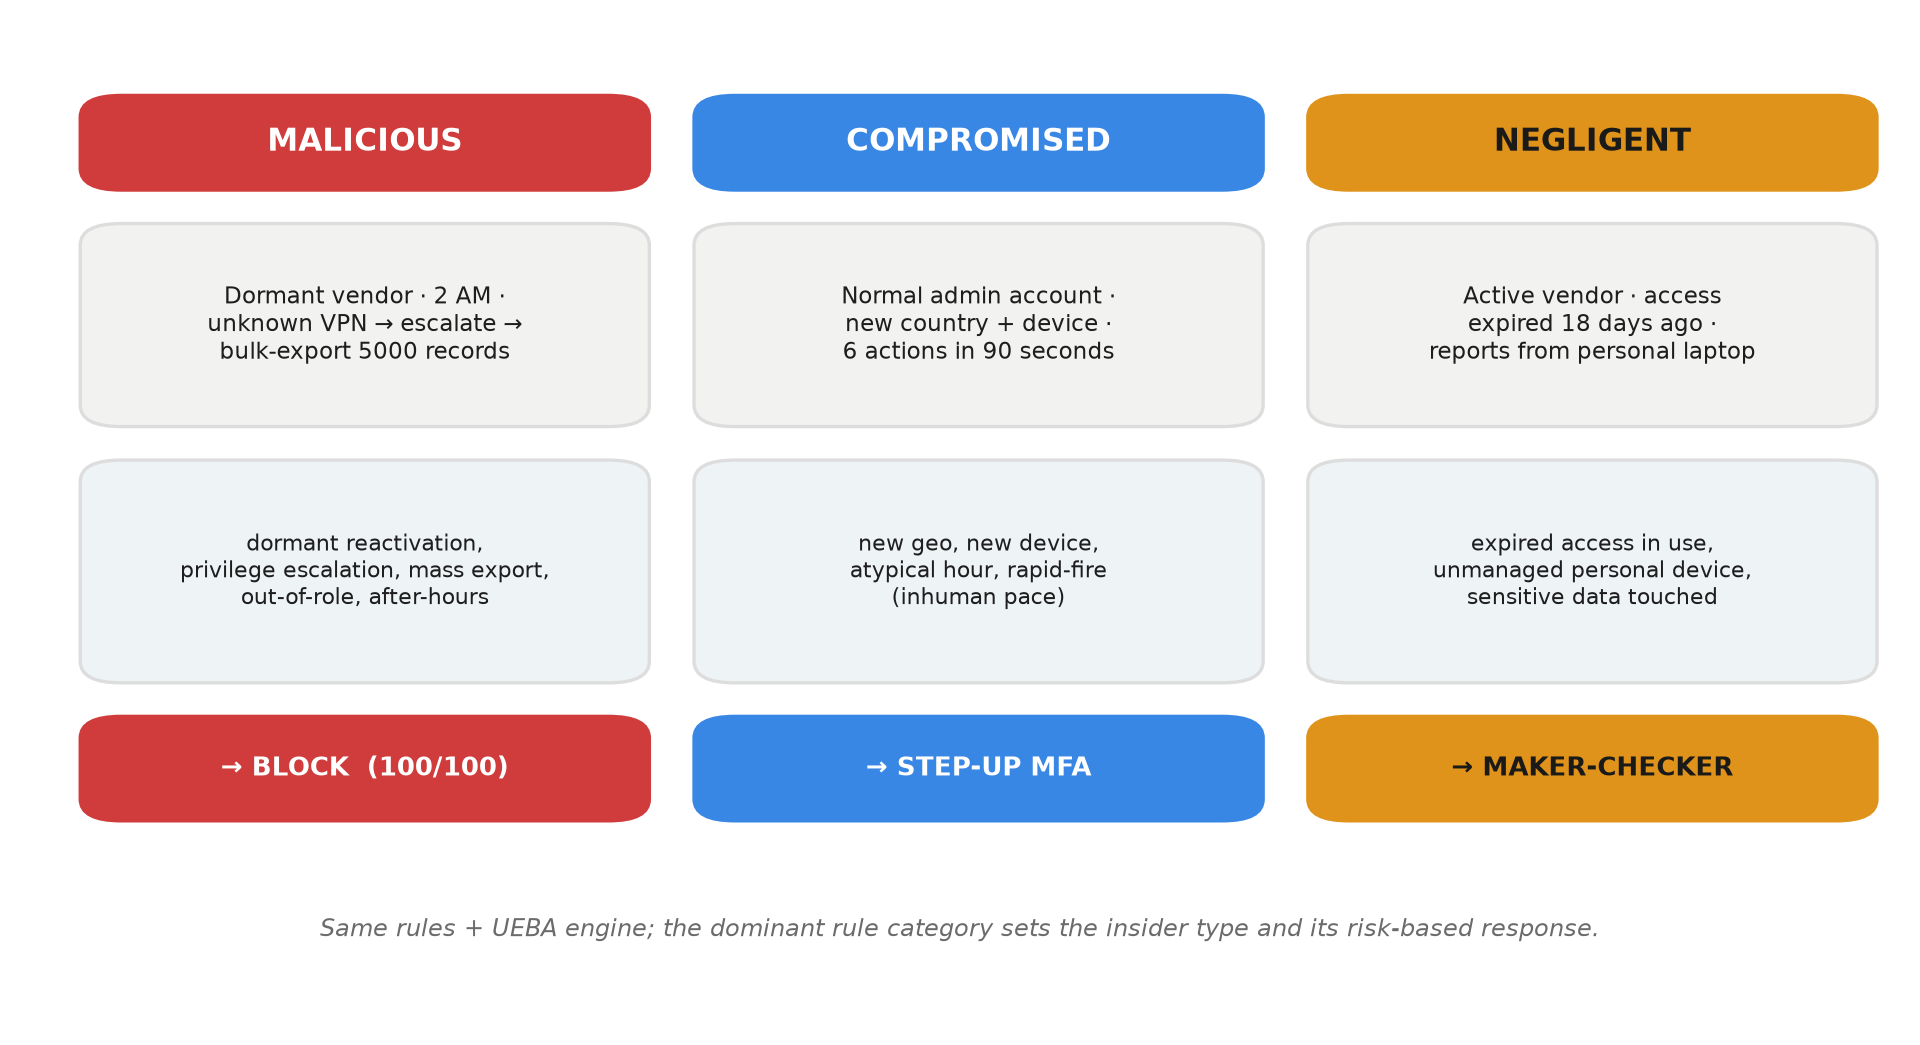
\includegraphics[width=1\linewidth,height=\textheight,keepaspectratio,alt={Three insider types --- one engine, three distinct, correctly-typed responses.}]{img/insider_types.png}
\caption{Three insider types --- one engine, three distinct,
correctly-typed responses.}
\end{figure}

{\def\LTcaptype{none} % do not increment counter
\begin{longtable}[]{@{}
  >{\raggedright\arraybackslash}p{(\linewidth - 6\tabcolsep) * \real{0.2500}}
  >{\raggedright\arraybackslash}p{(\linewidth - 6\tabcolsep) * \real{0.2500}}
  >{\raggedright\arraybackslash}p{(\linewidth - 6\tabcolsep) * \real{0.2500}}
  >{\raggedright\arraybackslash}p{(\linewidth - 6\tabcolsep) * \real{0.2500}}@{}}
\toprule\noalign{}
\begin{minipage}[b]{\linewidth}\raggedright
Scenario
\end{minipage} & \begin{minipage}[b]{\linewidth}\raggedright
Dominant signals
\end{minipage} & \begin{minipage}[b]{\linewidth}\raggedright
Score band
\end{minipage} & \begin{minipage}[b]{\linewidth}\raggedright
Response
\end{minipage} \\
\midrule\noalign{}
\endhead
\bottomrule\noalign{}
\endlastfoot
\textbf{Malicious} & dormant + escalation + mass-export + out-of-role +
after-hours & \textgreater= 85 & \textbf{BLOCK} \\
\textbf{Compromised} & new geo + new device + atypical hour + rapid-fire
& 40--69 & \textbf{STEP-UP MFA} \\
\textbf{Negligent} & expired access + unmanaged device & 70--84 &
\textbf{MAKER-CHECKER} \\
\end{longtable}
}

\textbf{Type-aware policy.} Negligence is a control failure to remediate
with a \textbf{human second-check}, not an attack to hard-block --- so a
negligent session is \textbf{floored to maker-checker review} and
\textbf{never escalated to an automated block}. Malicious blocks;
compromised steps up. This is enforced in
\texttt{decide(score,\ insider\_type)}.

\section{Adaptive Response and PAM}\label{adaptive-response-and-pam}

\subsection{Live enforcement}\label{live-enforcement}

Each portal action re-scores the \textbf{whole session including the
candidate action}, then enforces the decision \textbf{before the action
takes effect}.

\begin{figure}
\centering
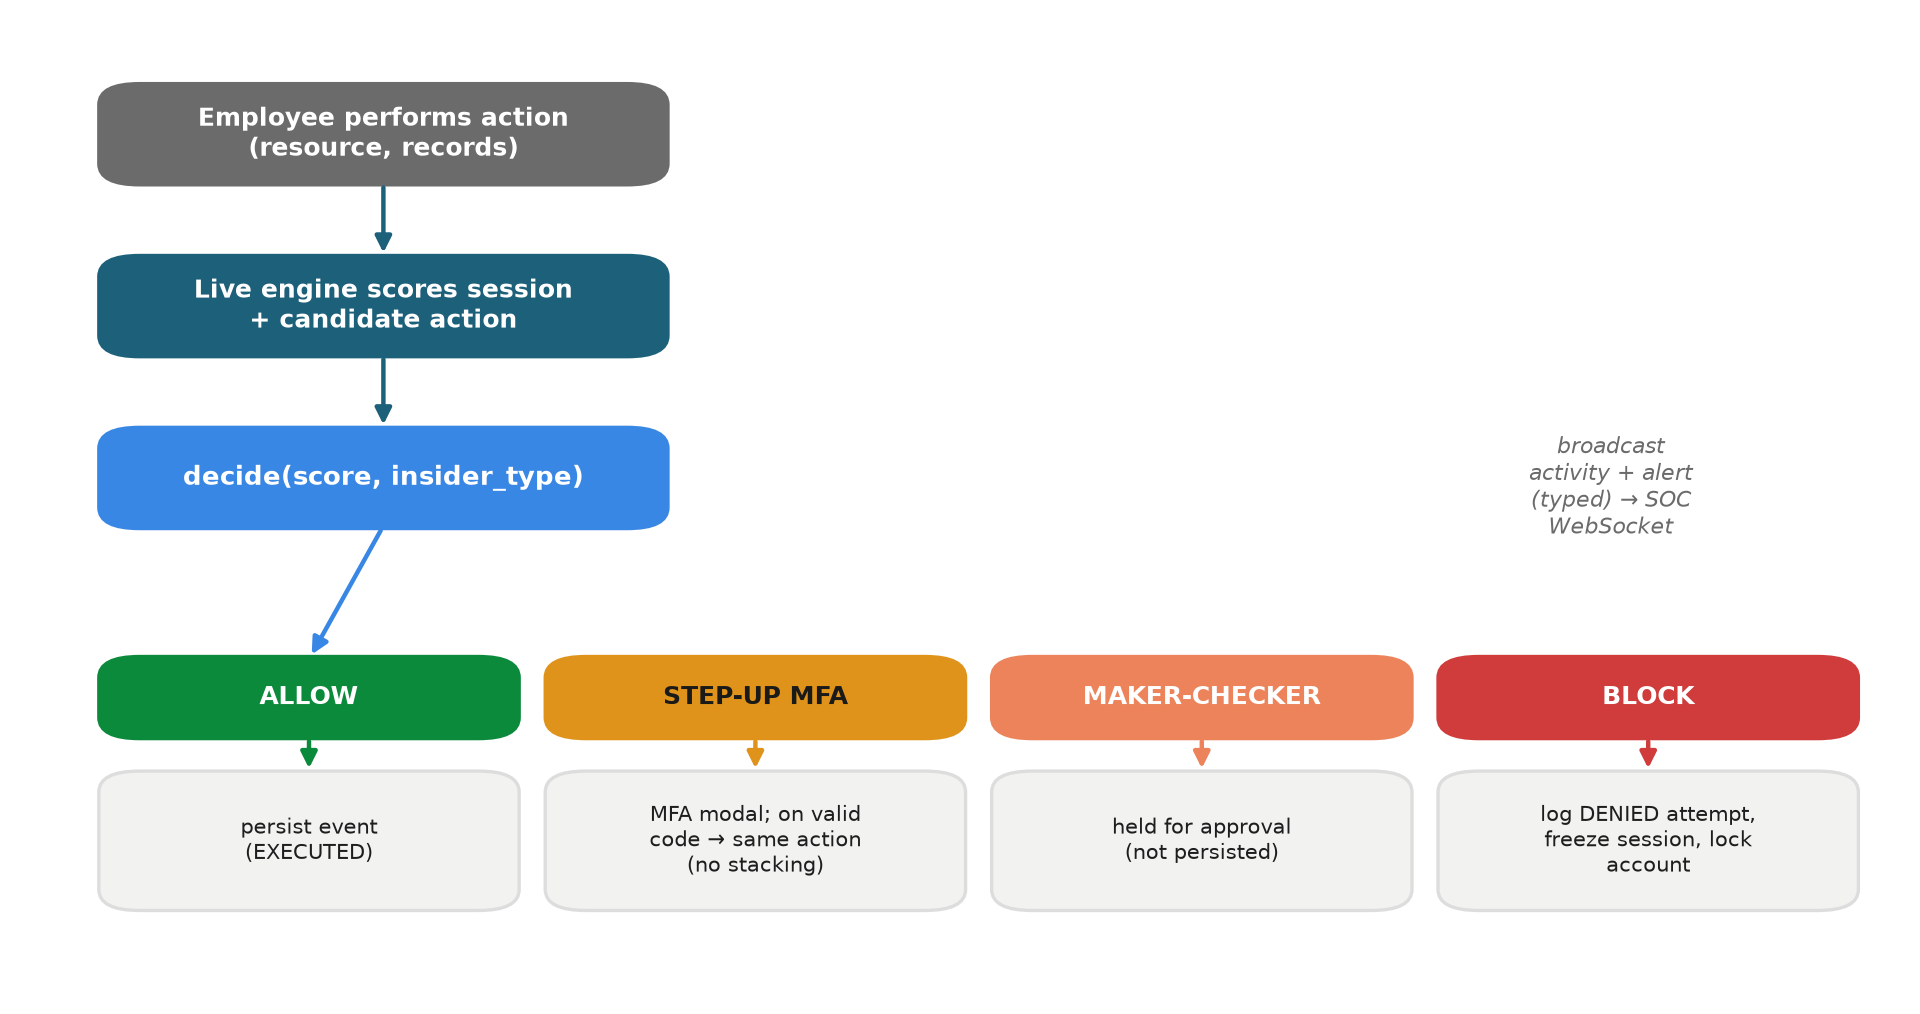
\includegraphics[width=1\linewidth,height=\textheight,keepaspectratio,alt={Live enforcement --- every action is scored and routed to one of four responses before it takes effect.}]{img/live_sequence.png}
\caption{Live enforcement --- every action is scored and routed to one
of four responses before it takes effect.}
\end{figure}

Key safety properties:

\begin{itemize}
\tightlist
\item
  \textbf{Blocked accounts stay locked.} A blocked session is returned
  on re-login; a blocked user cannot open a fresh session to continue.
\item
  \textbf{No score-gaming.} Challenged actions (MFA or maker-checker)
  are \textbf{not persisted} until actually allowed, so retrying does
  not inflate the session.
\item
  \textbf{Server-side enforcement.} The API refuses to execute; the UI
  overlay is cosmetic.
\end{itemize}

\subsection{PAM surface}\label{pam-surface}

\begin{itemize}
\tightlist
\item
  \textbf{Privileged-session recording}
  (\texttt{GET\ /soc/sessions/\{id\}/commands}) --- the replayable
  command trail; blocked commands show as DENIED (struck through), held
  ones as HELD.
\item
  \textbf{Access review} (\texttt{GET\ /soc/access-review}) --- every
  privileged account with standing-risk flags (DORMANT / VENDOR /
  EXPIRED) and a risk rating, surfacing lingering access \emph{before}
  anything happens.
\item
  \textbf{Maker-checker approval}
  (\texttt{POST\ /soc/sessions/\{id\}/approve}) --- an analyst approves
  a held session; the approval is written to the signed audit log.
\end{itemize}

\section{Post-Quantum Security Layer}\label{post-quantum-security-layer}

All post-quantum operations sit behind one abstraction,
\texttt{app/security/pqc.py}, exposing \texttt{kem\_keypair},
\texttt{kem\_encapsulate}, \texttt{kem\_decapsulate}, \texttt{sign}, and
\texttt{verify} over \textbf{ML-KEM-768} (FIPS 203) and
\textbf{ML-DSA-65} (FIPS 204).

\subsection{Credential vault}\label{credential-vault}

\begin{figure}
\centering
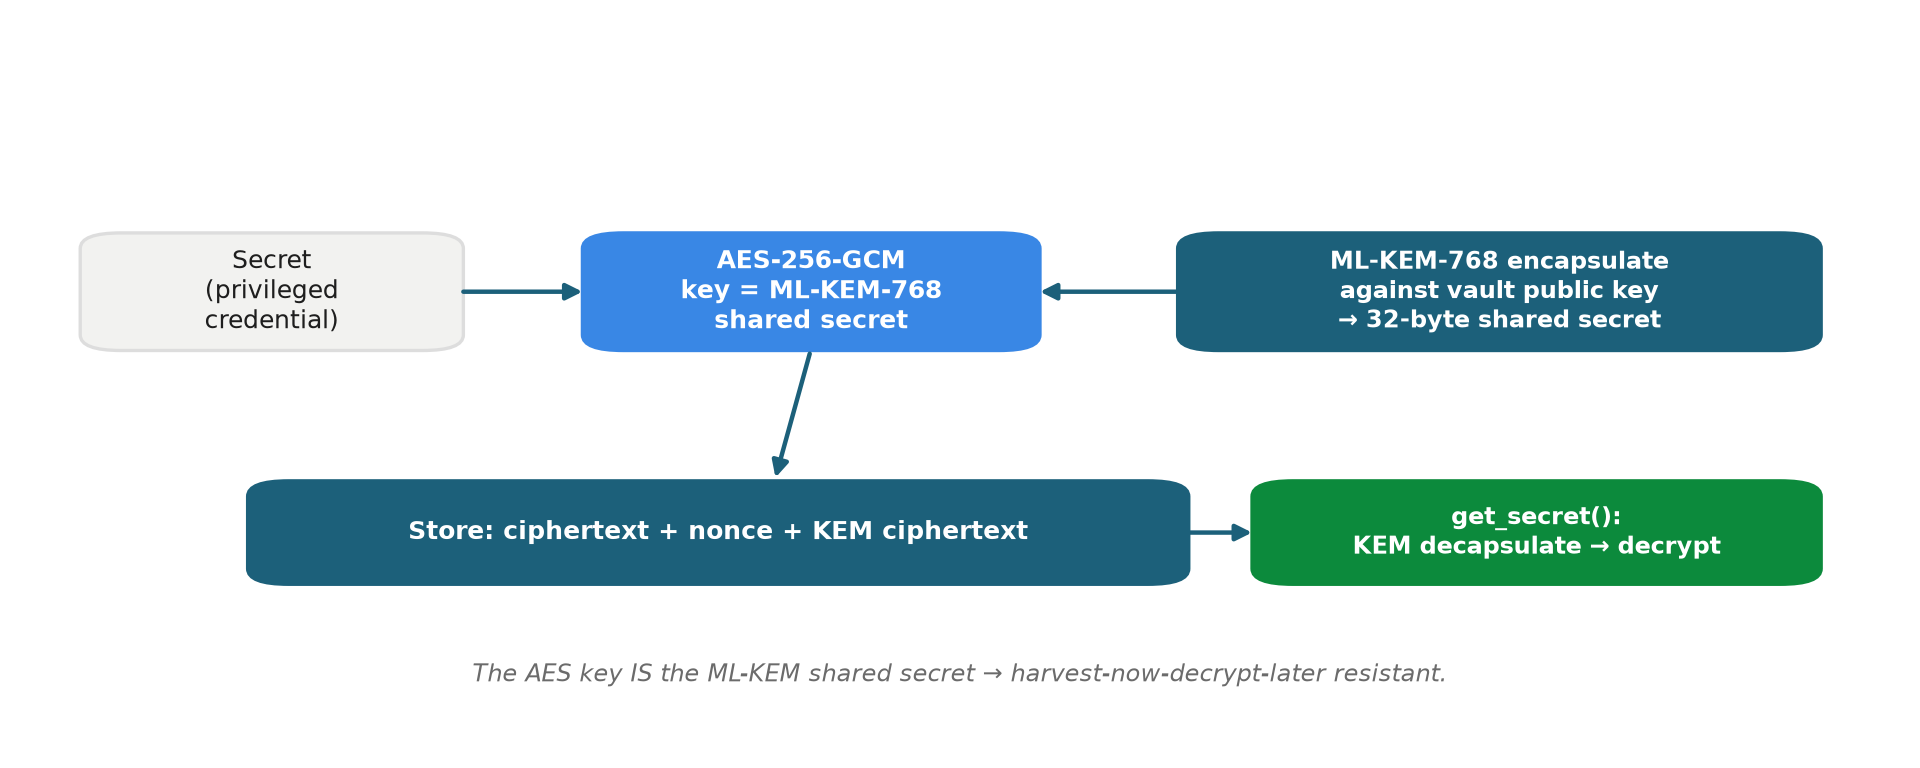
\includegraphics[width=0.95\linewidth,height=\textheight,keepaspectratio,alt={Credential vault --- a secret is sealed with AES-256-GCM under an ML-KEM-768 shared secret.}]{img/pqc_vault.png}
\caption{Credential vault --- a secret is sealed with AES-256-GCM under
an ML-KEM-768 shared secret.}
\end{figure}

The AES key \textbf{is} the ML-KEM shared secret; decryption requires
the vault's KEM secret key. Data recorded today cannot be decrypted
later, even by a quantum adversary.

\subsection{Tamper-evident audit log}\label{tamper-evident-audit-log}

\begin{figure}
\centering
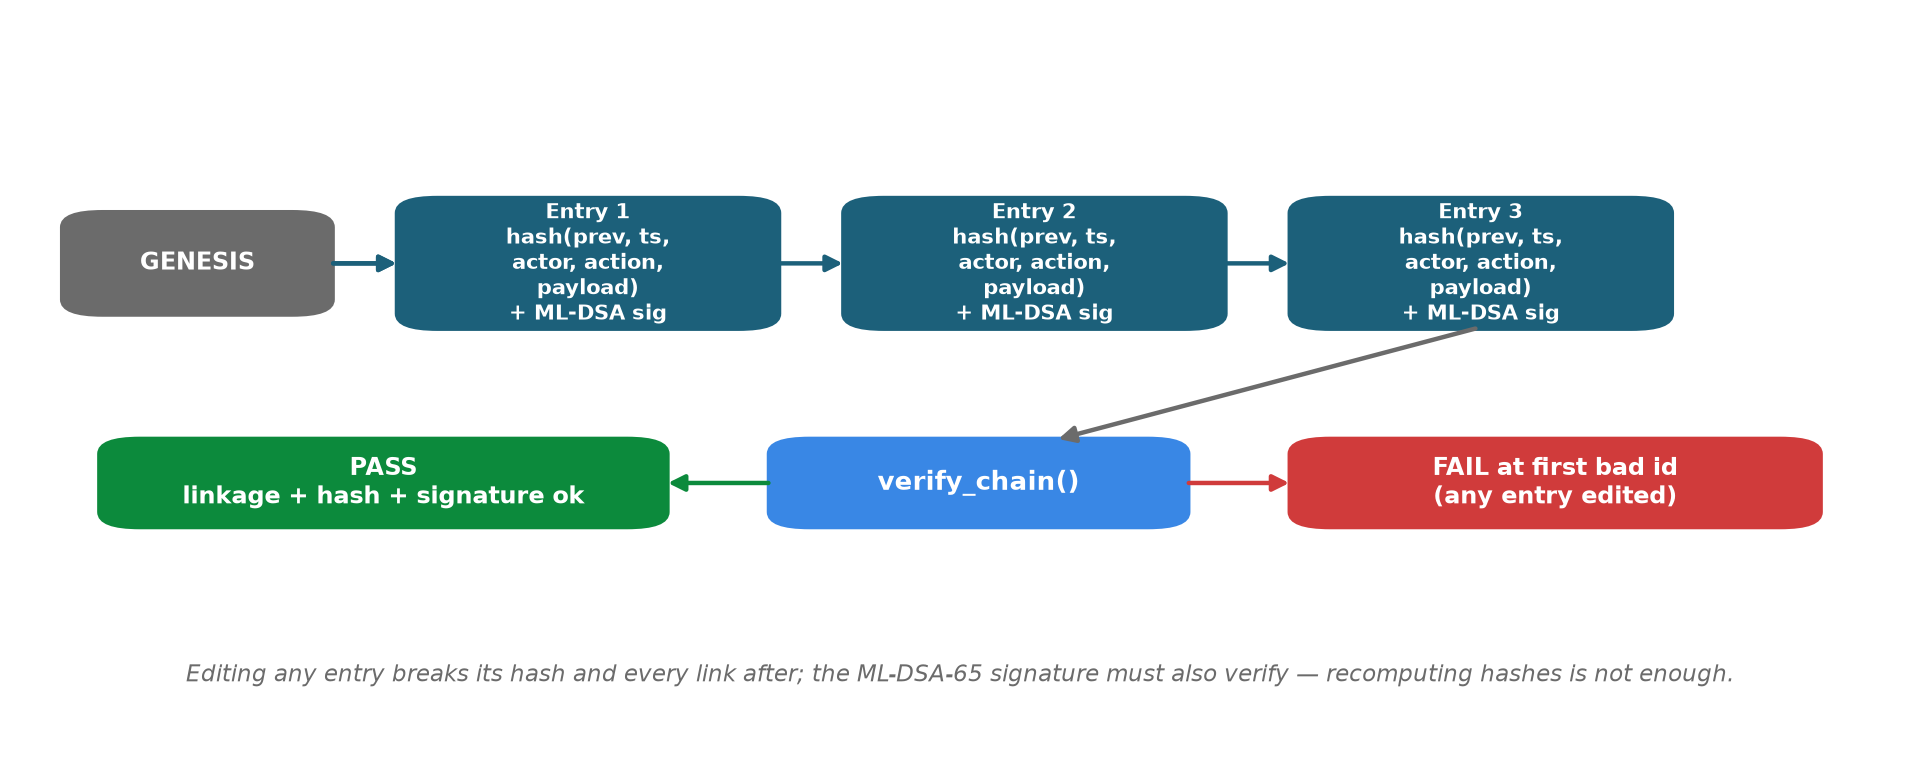
\includegraphics[width=0.95\linewidth,height=\textheight,keepaspectratio,alt={Audit chain --- each entry hash-links the previous and is ML-DSA-65 signed; any edit fails verification.}]{img/audit_chain.png}
\caption{Audit chain --- each entry hash-links the previous and is
ML-DSA-65 signed; any edit fails verification.}
\end{figure}

Each entry hash-chains the previous entry \textbf{and} is ML-DSA-65
signed. Editing any entry breaks its hash and every subsequent link;
recomputing hashes is not enough, because the signature must still
verify with the audit public key. \texttt{POST\ /demo/tamper} flips one
record live, and \texttt{verify\_chain()} then fails at the exact entry.

\section{Authentication and
Authorization}\label{authentication-and-authorization}

\begin{itemize}
\tightlist
\item
  \textbf{Passwords} --- PBKDF2-HMAC-SHA256 (200,000 rounds, per-user
  salt), in \texttt{app/security/auth.py}.
\item
  \textbf{Tokens} --- compact HMAC-SHA256-signed, JWT-like tokens with
  expiry, verified on every request.
\item
  \textbf{Roles} --- \texttt{EMPLOYEE} routes to the Employee Portal;
  \texttt{ANALYST} routes to the SOC Console. SOC endpoints are gated
  with \texttt{require\_analyst} (HTTP 403 for employees). The WebSocket
  feed is broadcast-only.
\end{itemize}

This layer is demo-grade by design; a production deployment swaps in the
bank's IdP/SSO behind the same dependency.

\section{API Reference}\label{api-reference}

{\def\LTcaptype{none} % do not increment counter
\begin{longtable}[]{@{}
  >{\raggedright\arraybackslash}p{(\linewidth - 6\tabcolsep) * \real{0.2500}}
  >{\raggedright\arraybackslash}p{(\linewidth - 6\tabcolsep) * \real{0.2500}}
  >{\raggedright\arraybackslash}p{(\linewidth - 6\tabcolsep) * \real{0.2500}}
  >{\raggedright\arraybackslash}p{(\linewidth - 6\tabcolsep) * \real{0.2500}}@{}}
\toprule\noalign{}
\begin{minipage}[b]{\linewidth}\raggedright
Method
\end{minipage} & \begin{minipage}[b]{\linewidth}\raggedright
Endpoint
\end{minipage} & \begin{minipage}[b]{\linewidth}\raggedright
Auth
\end{minipage} & \begin{minipage}[b]{\linewidth}\raggedright
Purpose
\end{minipage} \\
\midrule\noalign{}
\endhead
\bottomrule\noalign{}
\endlastfoot
POST & /auth/login & -- & issue token (username / password) \\
GET & /auth/me & any & current identity \\
POST & /portal/bootstrap & employee & open live session + catalog +
resources \\
POST & /portal/action & employee & perform action -\textgreater{} scored
and enforced \\
POST & /portal/logout & employee & close session \\
GET & /soc/overview & analyst & users, scored history, heatmap, live
sessions \\
GET & /soc/live & analyst & active / blocked sessions (typed) \\
GET & /soc/alerts & analyst & recent alerts (typed) \\
GET & /soc/access-review & analyst & PAM dormant / vendor / expired
table \\
GET & /soc/sessions/\{id\}/commands & analyst & session recording
replay \\
GET & /soc/sessions/\{id\}/events & analyst & session events \\
POST & /soc/sessions/\{id\}/approve & analyst & maker-checker
approval \\
POST & /demo/scenario/\{kind\} & analyst & run scripted malicious /
compromised / negligent \\
POST & /demo/tamper & analyst & edit an audit entry (proves
detection) \\
GET & /audit, /audit/verify & analyst & list / verify the signed
chain \\
GET & /pqc/info & any & active PQC provider and algorithms \\
POST, GET & /vault/secrets & analyst & store / retrieve a PQC-wrapped
secret \\
WS & /ws/feed & -- & live activity / alert / tamper frames \\
GET & /health & -- & liveness \\
\end{longtable}
}

Interactive API docs are served at \texttt{/docs} (FastAPI / OpenAPI).

\section{Frontend}\label{frontend}

React 19 + Vite + Tailwind 4, dark SOC theme, served by FastAPI from
\texttt{frontend/dist} (same-origin, offline).

\begin{itemize}
\tightlist
\item
  \textbf{Login} (\texttt{pages/Login.jsx}) --- role-routed, with a
  demo-account helper.
\item
  \textbf{Employee Portal} (\texttt{pages/Portal.jsx}) --- action
  console, connection badge, live risk gauge, activity timeline, MFA
  modal, maker-checker banner, and a full-screen BLOCK overlay.
\item
  \textbf{SOC Console} (\texttt{pages/SocConsole.jsx}) --- three
  scenario buttons, an audit banner, and panels: live sessions (typed),
  risk gauge, why-flagged, alerts (typed), timeline, session recording
  (terminal replay), heatmap, and access review.
\end{itemize}

The colour system reserves status colours (good / warning / serious /
critical), colour-codes insider types (malicious red, compromised blue,
negligent amber), uses tabular numerics, flashes on new alerts, and
never encodes meaning by colour alone.

\section{Security Considerations}\label{security-considerations}

\begin{itemize}
\tightlist
\item
  \textbf{Data minimization} --- scores on privileged-activity metadata;
  no customer PII required.
\item
  \textbf{Credential protection} --- an ML-KEM-768-wrapped AES-256-GCM
  vault for privileged secrets.
\item
  \textbf{Audit integrity} --- hash-chained and ML-DSA-65-signed
  entries; tampering is cryptographically evident.
\item
  \textbf{Enforcement} --- server-side; blocked accounts stay locked; a
  challenged action is not persisted until actually allowed (no
  score-gaming, no bypass by re-login).
\item
  \textbf{Authorization} --- role-gated APIs; analyst-only SOC and PQC
  endpoints.
\item
  \textbf{Offline by design} --- no external calls at runtime; keys kept
  out of version control; \texttt{.env}-driven configuration;
  least-privilege demo accounts.
\item
  \textbf{Explainability and compliance} --- every decision has a
  plain-English reason, an immutable trail, and access reviews for
  standing, dormant and expired grants.
\end{itemize}

\section{Scalability}\label{scalability}

\begin{itemize}
\tightlist
\item
  \textbf{Stateless scoring} --- scale horizontally behind a load
  balancer; each request scores one session.
\item
  \textbf{Storage} --- SQLite to PostgreSQL by changing one connection
  string (pure ORM, no raw SQL).
\item
  \textbf{Real-time fan-out} --- WebSocket behind a Redis or Kafka
  broker to serve many SOC clients and high event throughput.
\item
  \textbf{Ingestion} --- generalizes to enterprise PAM/SIEM feeds
  (millions of privileged events per day) on the same \texttt{Event}
  schema.
\item
  \textbf{Machine learning} --- models retrain per role and shift
  nightly; a feature store holds baselines; the UEBA interface accepts
  an autoencoder upgrade with no application changes.
\item
  \textbf{Post-quantum operations} --- ML-KEM encapsulation and ML-DSA
  signing are sub-millisecond, negligible next to a database write.
\end{itemize}

\section{Deployment and Running}\label{deployment-and-running}

\begin{Shaded}
\begin{Highlighting}[]
\CommentTok{\# Windows PowerShell}
\OperatorTok{.}\NormalTok{\textbackslash{}run}\OperatorTok{.}\FunctionTok{ps1}              \CommentTok{\# venv + deps + seeded DB + UI + API (offline)}
\OperatorTok{.}\NormalTok{\textbackslash{}run}\OperatorTok{.}\FunctionTok{ps1} \OperatorTok{{-}}\NormalTok{Reset       }\CommentTok{\# wipe and reseed for a clean demo}
\end{Highlighting}
\end{Shaded}

\begin{Shaded}
\begin{Highlighting}[]
\CommentTok{\# Git Bash / Linux / macOS}
\ExtensionTok{./run.sh}               \CommentTok{\# same, POSIX}

\ExtensionTok{docker}\NormalTok{ compose up }\AttributeTok{{-}{-}build}      \CommentTok{\# container alternative}
\end{Highlighting}
\end{Shaded}

Then open \texttt{http://127.0.0.1:8000}. The first run on a fresh
machine needs internet once (pip install plus a one-time liboqs build);
afterwards it is fully offline. Run tests with
\texttt{.venv/Scripts/python\ -m\ pytest}.

\section{Testing}\label{testing}

The suite contains \textbf{31 pytest tests}, including:

\begin{itemize}
\tightlist
\item
  \textbf{test\_simulator} --- user seeding, normal-day realism,
  determinism.
\item
  \textbf{test\_detection} --- every rule, normal-versus-attack scoring,
  quiet-on-normal.
\item
  \textbf{test\_scenarios} --- the three insider scenarios land on
  distinct, correct paths and the type-aware policy holds (negligence
  never auto-blocks), on an independent seed.
\item
  \textbf{test\_phase3} --- attack block, alert, and the WebSocket loop.
\item
  \textbf{test\_portal} --- authentication, role gating, live
  enforcement, MFA without event stacking, and blocked-stays-locked.
\item
  \textbf{test\_pqc} --- KEM round-trip, sign/verify with forgery
  rejection, vault round-trip, and audit chain clean / tamper /
  signature-forgery.
\end{itemize}

\section{Demo Walkthrough}\label{demo-walkthrough}

Full narration is in \texttt{DEMO\_SCRIPT.md}. In brief (two browser
windows, side by side):

\begin{enumerate}
\def\labelenumi{\arabic{enumi}.}
\tightlist
\item
  \textbf{SOC Console} (\texttt{soc\_admin}) --- quiet, with a green
  heatmap.
\item
  \textbf{Employee Portal} (\texttt{rmehta}) --- a normal query is
  ALLOWED; an export of 1000 records triggers STEP-UP MFA (code
  \texttt{246810}).
\item
  \textbf{Attacker} (\texttt{ext\_dsouza}) --- escalate then export 5000
  records -\textgreater{} full-screen BLOCK; the account is locked.
\item
  \textbf{SOC lights up} --- a red live session at 100, a flashed
  CRITICAL alert tagged \texttt{malicious}, the why-flagged panel, the
  session replay (export struck through as DENIED), and a red heatmap
  cell.
\item
  \textbf{Two more insider types} --- the SOC buttons run Compromised
  -\textgreater{} MFA and Negligent -\textgreater{} maker-checker, each
  correctly typed.
\item
  \textbf{PAM access review} --- dormant, vendor and expired flags.
\item
  \textbf{Quantum-safe evidence} --- Verify Chain (green) then Tamper
  (red, FAILED at the exact entry).
\end{enumerate}

\section{Roadmap}\label{roadmap}

\begin{itemize}
\tightlist
\item
  \textbf{PS2 correlation} --- link a privileged record-change to a
  suspicious downstream transaction.
\item
  \textbf{Just-in-time access} and automated entitlement reviews.
\item
  \textbf{Autoencoder} UEBA upgrade behind the same interface.
\item
  \textbf{Enterprise integrations} --- CyberArk / BeyondTrust PAM,
  Splunk / QRadar SIEM, IdP / SSO.
\item
  \textbf{Workforce-wide insider-risk scoring} beyond privileged
  accounts.
\end{itemize}

\section{Repository Map}\label{repository-map}

\begin{verbatim}
PRAHARI/
  app/
    main.py               FastAPI app + lifespan + static UI mount
    config.py             pydantic settings (.env)
    pam.py                session-command recording + access review
    api/routes.py         REST + WebSocket endpoints
    api/ws.py             WebSocket broadcast manager
    detection/rules.py    rule engine (3 insider types, typed)
    detection/ueba.py     IsolationForest + peer baseline (prefix-trained)
    detection/score.py    0-100 risk score + reasons + insider type
    detection/response.py type-aware adaptive response
    detection/live.py     live per-action scoring & enforcement
    models/entities.py    ORM entities
    security/auth.py      PBKDF2 passwords + HMAC tokens
    security/pqc.py       ML-KEM-768 / ML-DSA-65 abstraction
    security/vault.py     quantum-safe credential vault
    security/audit.py     hash-chained + signed audit log
    simulator/            normal-day generator, 3 scenarios, seeder
  frontend/               React app (pages/ + components/) + prebuilt dist/
  tests/                  31 pytest tests
  docs/                   this documentation + submission deck
  DOCUMENTATION.md  DEMO_SCRIPT.md  PROJECT_STATUS.md  README.md
  run.ps1  run.sh  Dockerfile  docker-compose.yml  requirements.txt
\end{verbatim}

\emph{Prahari --- the sentinel for privileged access. Detect with AI and
rules, explain every decision, respond in real time, and keep the proof
quantum-safe.}

\end{document}
